\documentclass[12pt,a4paper]{article}
\usepackage[utf8]{inputenc}%agregado
\usepackage{amsmath}
\usepackage{graphicx}
\usepackage{amssymb}%agregado
\usepackage{amsthm}%agregado
\usepackage{color}	

%---
\usepackage[breaklinks=true,backref=page]{hyperref}

\usepackage[english]{babel}%agregado
%\usepackage{natbib}%agregado para ref apa
\usepackage[square,numbers]{natbib}%agregado ref apa

%\usepackage[section,nottoc]{tocbibind}%poner referenica en la tabla de contenidos
\usepackage[nottoc]{tocbibind}%poner referenica en la tabla de contenidos



\usepackage{amsthm}
%\theoremstyle{plain}
%\newtheorem{thm}{Teorema}[section]
%\newtheorem{lem}[thm]{Lema}
%\newtheorem{prop}[thm]{Proposición}
%\newtheorem{cor}[thm]{Corolario}
\theoremstyle{plain}% default
\newtheorem{thm}{Theorem}[section]
\newtheorem{lem}[thm]{Lemma}
\newtheorem{prop}[thm]{Proposition}
\newtheorem*{cor}{Corollary}
%\newtheorem*{KL}{Klein’s Lemma}

\theoremstyle{definition}
\newtheorem{defn}{Definición}[section]
%\newtheorem{conj}{Conjectura}[section]
\newtheorem{exmp}{Ejemplo}[section]
\newtheorem{xca}[exmp]{Ejercicio}

\theoremstyle{remark}
\newtheorem*{rem}{Observación}
\newtheorem*{note}{Note}
\newtheorem{case}{Case}







%\title{Distribución de parásitos por sexo y la probabilidad de apareamiento}
\title{Basic modeling water sanitation and hygiene impacts over the transmission of soil-transmitted helminths}
\author{Gonzalo Maximiliano LOPEZ$^{1,3,4}$, Juan Pablo APARICIO$^{1,2}$\\
	\\
	{\small $^1$ Instituto de Investigaciones en Energ\'ia no Convencional (INENCO),} \\ {\small Consejo Nacional de Investigaciones Cient\'ificas y T\'ecnicas (CONICET),}\\
	{\small Universidad Nacional de Salta, Av. Bolivia 5150, 4400 Salta, Argentina.}\\
	$^2${\small Simon A. Levin Mathematical, Computational and Modeling Sciences Center,} \\ {\small Arizona State University, PO Box 871904 Tempe, AZ 85287-1904, USA}\\
	{\small $^3$ Departamento de Matem\'atica,}\\{\small Universidad Nacional de Salta, Av. Bolivia 5150, 4400 Salta, Argentina.}\\
	{\small $^4$ Corresponding author: gonzalo.maximiliano.lopez@gmail.com}}
\date{}



\begin{document}

\maketitle

\begin{abstract}
	\addcontentsline{toc}{section}{Abstract}
	Completar
	
	Keywords: mathematical modeling; soil-transmitted helminths; water sanitation and hygiene
\end{abstract}

\tableofcontents



\section{Introduction}
{\color{red}
%• First, you need to have a thorough knowledge about everything that has been
%	previously written on the topic and decide what is important for the reader to
%	know.
%	
%	• Then, you have to give the reader the tools for understanding the meaning and
%	motivation of your experiments.
%	
%	• Finally, tell your readers how you plan to develop your topic. Give them a
%	roadmap to follow - show them what your line of argument is.}
%
%{\color{red}
	Las helmintiasis transmitidas por el contacto con el suelo, conocidas como geohelmintiasis, son las infecciones más comunes a nivel mundial y afectan a las poblaciones más pobres y vulnerables. 
	%La infección se produce por la ingestión de huevos infectantes procedentes de tierra contaminada con heces humanas, o de productos agrícolas crudos contaminados con tierra que contenga huevos infectantes (A. lumbricoides y T. trichiura) o por la penetración de larvas desde el suelo a través de la piel (uncinarias).
	Estas se transmiten por huevos de los parásitos presentes en las heces humanas que contaminan el suelo en las zonas con deficientes sistemas de saneamiento.
	
	Los agentes causales de esta infección son los nematodos (\textit{Ascaris lumbricoides}, \textit{Trichuris trichiura}) y las uncinarias (\textit{Necator americanus} y \textit{Ancylostoma duodenale}), los cuales infectan a los humanos a través de la ingesta de alimentos contaminados con sus huevos, o por la penetración de larvas desde el suelo a través de la piel (larvas de \textit{Ancylostoma}) principalmente al andar descalzos en el suelo contaminado.
	
	%Los agentes causales son \textit{Ascaris lumbricoides}, \textit{Trichuris trichiura} y las uncinarias (\textit{Necator
	%americanus} y \textit{Ancylostoma duodenale}). 
	
	En las Américas, las helmintiasis transmitidas por el contacto con el suelo están presentes en toda la Región.
	Se estima que una de cada tres personas está infectada por geohelmintos y cerca de 46 millones de niños entre 2 y 14 años están en riesgo de infectarse por estos parásitos, aproximadamente 13 millones de niños en edad pre-escolar (2 a 4 años) y 33,3 millones en edad escolar (de 5 a 14 años) \cite{paho2003,who2006preventive,who2012soil}.
	%, por falta de saneamiento básico y acceso a agua potable. 
	%La infección es más frecuente en mujeres y niños. 
	%La falta de acceso a agua y saneamiento es la causa de la persistencia de estas infecciones. 
	
	Los principales factores de riesgo para la ocurrencia de infecciones por geohelmintos están relacionados con la falta de acceso al agua potable segura,  saneamiento básico y pobres condiciones higiénicas y de vivienda.  La eliminación apropiada de los desechos humanos es especialmente crítica, ya que un gramo de heces puede contener hasta 100 huevos de parásitos. Por consiguiente, los suministros de agua contaminados pueden infectar y reinfectar a las personas de todo un pueblo o toda una aldea \cite{paho2003,who2006preventive,who2012soil}.
	
	%La desparasitación masiva una o dos veces al año en comunidades y países con altas prevalencias, junto con medidas de higiene personal, e incremento al acceso a agua y saneamiento son las intervenciones para reducir la carga de enfermedad.




Las infecciones por geohelmintos se tratan con fármacos de administración oral siendo los más comunes Albendazol y Mebendazol,
 %medicamentos antihelmínticos
   que se distribuyen a las poblaciones afectadas en campañas o programas de desparasitación masiva (PDM). Comúnmente estas campañas están dirigidas a las poblaciones más afectadas,  niños de 2 a 14 años de edad \citep{pizzi2007geohelmintiosis}. 
%Además del tratamiento con antihelmínticos, estudios recientes también demuestran que la combinación de agua potable segura, instalaciones de saneamiento adecuadas y buenas prácticas de higiene (\textit{WASH} por sus siglas en ingles) junto con las campañas de AMM reducen la reinfección por geohelmintos \cite{strunz2014water}.

Además del tratamiento con antihelmínticos, estudios recientes también demuestran que la combinación de acceso al agua potable segura, instalaciones de saneamiento adecuadas y buenas prácticas de higiene 
que denotaremos por \textit{WASH} (por sus siglas en ingles) 
junto con los PDM reducen la reinfección por geohelmintos \cite{strunz2014water}.
Las intervenciones  WASH son diversas y pueden incluir mejoras en el acceso al agua (p. ej. calidad del agua, cantidad de agua y distancia al agua), acceso al saneamiento (p. ej. acceso a letrinas mejoradas, mantenimiento de letrinas y gestión de lodos fecales) y prácticas de higiene (p. ej. lavado de manos antes de comer y después de defecar, tratamiento del agua, uso de jabón, uso de calzado y prácticas de almacenamiento de agua). 
%Las intervenciones a menudo incluyen múltiples componentes, por ejemplo, la construcción de letrinas de pozo mejoradas con ventilación y al mismo tiempo se brinda educación sobre higiene.	
%junto con programas de STH (es decir, campañas de MDA) reducen la reinfección de STH (Strunz et al. 2014).

%Además del tratamiento con antihelmínticos, estudios recientes también demuestran que las intervenciones

%la intervención de agua potable segura, instalaciones de saneamiento adecuadas y buenas prácticas de higiene que llamaremos  


%\textit{WASH} (por sus siglas en ingles) en combinación con los PDM reducen la reinfección por geohelmintos \cite{strunz2014water}.

En este capítulo analizamos el impacto de las intervenciones WASH en las geohelmintiasis en diferentes contextos epidemiológicos con y sin PDM. 
Tanto los modelos deterministas como los estocásticos se han aplicado ampliamente para estudiar la dinámica de transmisión de los geohelmintos en varios escenarios \cite{anderson1985community,anderson1992infectious,anderson2014coverage,truscott2014modeling,truscott2016soil}. Por lo tanto, utilizamos la idea general del modelado proporcionado en estos estudios anteriores e %al tiempo que 
incorporamos aspectos importantes adicionales al modelado, como la estructura demográfica por edades y la comparación del impacto de dos intervenciones (WASH y PDM).  
Para el caso del modelo determinista este está basado en ecuaciones diferenciales ordinarias con estructura de edades, mientras que  el estocásticos es un modelo basado en individuos (MBI), ambos desarrollados para analizar tanto la transmisión y control de geohelmintos.
%{\color{green} 
Nuestro objetivo en este capítulo es 
%Principalmente estamos interesados en 
determinar el impacto de las intervenciones  WASH y PDM sobre la carga media de parásitos y el tiempo de eliminación (es decir, el tiempo necesario para interrumpir la infección por geohelmintos) específicas de la dinámica de transmisión en la población de hospedadores.

}

%En este artículo desarrollamos un modelo matemático estructurado por edad basado en ecuaciones diferenciales ordinarias (ODE), que son parte de modelos deterministas, para determinar el impacto de las intervenciones de MDA y WASH en la carga de gusanos y el período de eliminación (es decir, el tiempo necesario para interrumpir STH transmisión) específicas de la dinámica de transmisión de la infección de Kenia. 

%Este análisis es abordado tanto por un modelo determinista como por un modelo estocástico.
%%Este impacto es estudiado tanto por un modelo determinista como por un modelo estocástico. 
%Para el determinista desarrollamos un modelo matemático de estructura de edades basado en ecuaciones diferenciales ordinarias.
%Los modelos deterministas se han aplicado ampliamente para estudiar la dinámica de transmisión de geohelmintos en varios entornos (ref ). Por lo tanto, utilizamos el marco de modelado proporcionado en estos estudios anteriores al tiempo que incorporamos aspectos importantes adicionales al modelo, como la estructura de edad completa y la comparación del impacto de dos intervenciones (MDA y WASH).  
%
%El modelo estocásticos es un modelo basado en individuos desarrollado para analizar tanto la transmisión y control de geohelmintos. 
  
%  la importancia relativa de la adopción (proporción de la población que asume la intervención) y la efectividad (impacto de las intervenciones en los individuos que asumen las intervenciones). Finalmente, investigamos el valor agregado de WASH a las estrategias actuales de control de STH, en particular para mantener los logros obtenidos a largo plazo.

%{\color{red}
%Para esta analizar desalloamos tanto un modelo determinista como un modeo estocasticoa . Para el primero de ellos desarrollamos un modelo matemático de estructura de edades basado en ecuaciones diferenciales ordinarias
%
%
%En este artículo desarrollamos un modelo matemático estructurado por edad basado en ecuaciones diferenciales ordinarias (ODE), que son parte de modelos deterministas, para determinar el impacto de las intervenciones de MDA y WASH en la carga de gusanos y el período de eliminación (es decir, el tiempo necesario para interrumpir STH transmisión) específicas de la dinámica de transmisión de la infección de Kenia. 

%Los modelos deterministas se han aplicado ampliamente para estudiar la dinámica de transmisión de STH en varios entornos (11, 16, 24–32). Por lo tanto, utilizamos el marco de modelado proporcionado en estos estudios anteriores al tiempo que incorporamos aspectos importantes adicionales al modelo, como la estructura de edad completa y la comparación del impacto de dos intervenciones (MDA y WASH). Predijimos el impacto a corto plazo (5 años) y a largo plazo (> 10 años) de las intervenciones bajo varios planes MDA para cada una de las tres especies de STH. 
%
%Los resultados de estos modelo serán importantes para el programa de control degeomintos ya que demostró claramente el impacto de las dos intervenciones clave en la carga de gusanos y el período de eliminación.
%
%de las STH de Kenia, así como para la OMS, ya que demostró claramente el impacto de las dos intervenciones clave en la carga de gusanos y el período de eliminación. Un resultado importante en este momento en que los programas de control están avanzando hacia el objetivo de la OMS de eliminar las STH para el año 2030 (33).
%
%
%, utilizando una extensión WASH recientemente desarrollada del marco de modelado de WORMSIM basado en individuos establecido para la transmisión y control de helmintos [15]. 
%
%Usamos el modelo para explicar primero los hallazgos del estudio W4W (es decir, ningún impacto notable de las letrinas en el contexto del PCT en toda la comunidad), luego predecir el impacto a corto y largo plazo de las diferentes modalidades de WASH y la importancia relativa de la adopción (proporción de la población que asume la intervención) y la efectividad (impacto de las intervenciones en los individuos que asumen las intervenciones). Finalmente, investigamos el valor agregado de WASH a las estrategias actuales de control de STH, en particular para mantener los logros obtenidos a largo plazo.	
%}
	
%\subsection{Intervención con \textit{WASH} en las poblaciones}
	
%	Conceptos modelo para WASH. Para fines de modelado, definimos dos modalidades de WASH: 1) intervenciones de "higiene" que reducen la exposición de las personas a las infecciones (por ejemplo, lavarse las manos y usar zapatos), y 2) intervenciones de "saneamiento" que reducen la contribución de las personas a la reservorio ambiental de infección (por ejemplo, uso de letrinas). La definición de estas dos modalidades no pretende excluir el "agua" en "WASH"; Consideramos que el agua es de importancia potencial para cualquiera de las modalidades dependiendo de para qué se necesita el agua, p. lavarse las manos (higiene
%	modalidad) o para descargar letrinas (modalidad de saneamiento). Además, definimos el impacto de WASH en términos de aceptación y eficacia. Aquí, la captación representa la proporción de la población que asume la intervención WASH, y la efectividad se define a nivel individual, es decir,
%	la reducción media de la exposición o la contribución a la transmisión a lo largo del tiempo, dado que un individuo asume la intervención hasta cierto punto (pero no necesariamente se beneficia de su máximo potencial debido, por ejemplo, a un uso irregular o inadecuado).
%	
%	
%	El impacto de las intervenciones de higiene se define por el término $1- ( H   H, i, t)$, que multiplicamos por el FOI i, t que actúa sobre un individuo en el mes t. Aquí, H, i, t es cero o uno, lo que representa si el individuo i asume o no la intervención en el mes t. La absorción individual  H, i, t está determinada por la absorción de la intervención a nivel de población general definida por el usuario (una fracción entre cero y uno) en el mes t y el índice de participación de WASH de un individuo, que es un número aleatorio de por vida entre cero y uno extraídos de una distribución uniforme:
%	H, i, t = 1 si el índice de participación del individuo es menor o igual que el nivel de captación total de la población, y  H, i, t = 0 en caso contrario. Como resultado, la captación de un individuo se considera constante en el tiempo si la captación a nivel de población es constante en el tiempo. La variación temporal a pequeña escala (por ejemplo, diaria) en la absorción real de la intervención se captura mediante el parámetro  H (también denominado "eficacia"), que representa la reducción promedio en FOI i, t a lo largo del tiempo en los individuos que toman el intervención, dado su cumplimiento y la calidad de la intervención. Como tal, los valores de  H cercanos a uno (reducción del 100%) probablemente no sean realistas. Además, se asume que la eficacia  H es la misma para todos los individuos que realizan la intervención.
%	Los diferentes tipos o combinaciones de intervenciones de higiene (por ejemplo, lavado de manos y / o calzado) solo se distinguen en términos de su aceptación y eficacia.
%	De manera similar a lo anterior, el impacto de las intervenciones de saneamiento (subíndice S en lugar de H) está representado por el término 1- ( S   S, i, t), que multiplicamos por la contribución de cada individuo al reservorio ambiental. Aquí, la absorción individual  S, i, t de las intervenciones de saneamiento se basa
	
	
	
%	Luego desarrollaron los aspectos de intervención WASH del modelo, en particular:
%	\begin{itemize}
%		\item Intervención del agua potable: reducción de la exposición de las hospedadores a la infección, por ejemplo mediante el lavado de manos, lavado de alimentos y consumo de agua potable.
%		\item Intervención del saneamiento: reducción de la contribución de las hospedadores al medio ambiente, por ejemplo mediante el uso de letrinas.
%	\end{itemize}
%	En términos del modelo la implemetciondel agua potable y saneamiento en al comunidad de hospedadores 
%	
	\section{Basic deterministic model with \textit{WASH} interventions}\label{sec:model1}
	\subsection{A homogeneous model}
	A basic model for soil-transmited helminth transmission was developed by Anderson and May in 1985  \citep{anderson1992infectious}. This model considers two variables, the mean burden of parasites in a host population (M) and the infectious environment formed by eggs or larvae of these parasites (L). The model is defined by a set of nonlinear ordinary differential equations as follows:
%	Un modelo básico para la transmisión de geohelmintos fue desarrollado por Anderson y May en 1985 \citep{anderson1992infectious}. 
%	Este modelo considera dos variables, la carga media de parásitos en una población (M) y 
%	el ambiente infeccioso formado por huevos y/o larvas de estos parásitos (L).
%	%la carga de huevos y/o larvas de estos parasitos (L).
%	%Este modelo consiste en la transmisión de esta infección  a través de dos estados, la carga media de parásitos de una población de hospedadores $M$ y el ambiente infeccioso formado por huevos y larvas de estos parásitos $L$.
%	El modelo está definido de la siguiente manera:   
%	%Para comenzar con este primer modelo supondremos que trabajamos sobre una población de hospedadores homogénea.  
%	%La dinámica temporal de la carga media de parásitos $M$ y la del material infeccioso formado por huevos y larvas presentes en el ambiente $L$ (o simplemente reservorio) viene dada por el siguiente sistema dinámico REF
	\begin{equation}\label{model1}
	\begin{split}
	\dfrac{dM}{dt}&=\beta L - (\mu_H+\mu_P) M\\
	\dfrac{dL}{dt}&= \alpha \lambda_0  \rho M F(M)  - \mu_L L 
	\end{split}
	\end{equation}
	%donde sus parámetros se describen a continuación:
	where the associated parameters are defined below:
	\begin{itemize}
		\item %$\beta$ y $\rho$ son las tasas de contacto (o exposición) y de aporte (o contribución) de un individuo con el reservorio $L$ (porción del reservorio per cápita) respectivamente
		$\rho$ and $\rho$ are the rate of contact (or exposure) and the rate contribution of a host to the reservoir $L$, respectively
		\item $\mu_H$, $\mu_P$ and $\mu_L$ 
		are the mortality rates associated with the host, the parasite and the reservoir, respectively
		%son las tasas de mortalidad asociadas al hospedador, los parásitos y el reservorio respectivamente
		%\item $\sigma$ la tasa de ingreso del material infeccioso, producido por las hembras, al reservorio
		\item $\alpha$ %la proporción de hembras en la población de parásitos
		the proportion of females in the parasite population
		\item $\lambda_0$ %la tasa de producción de huevos por hembra independiente de la densidad de parásitos en el hospedador
		the rate of egg production per female independent of host parasite density
		%\item $\pi_i$ la proporción de hospedadores del grupo $i$
		%\item $\epsilon_A$ y $\epsilon_S$ son los valores de eficacia de la intervención del agua potable y saneamiento respectivamente
		\item $F$ %{\color{green} %cuantifica los efectos de la fecundidad dependiente de la densidad	de los parásitos por hospedador y los efectos de la probabiliadad de apareamiento. 
		is the product of the functions: $\psi$ which quantifies the effects of the distribution of parasites in the host population and their fecundity dependent on the density of the parasites in the host; and $\phi$ which quantifies the effects of reproduction between parasites (mating probability) assuming a polygamous mating system. When the absence of density-dependence fecundity effects and mating probability is assumed, we assume that $F = 1$ (unit). As an example, if a negative binomial model is assumed for the distribution of parasites, the expressions for $\psi$ and $\rho$ are given by the expressions obtained in chapter 3,
		
		
		
		es el producto de las funciones: 
		$\psi$ que cuantifica los efectos de la distribución de parásitos en la población de hospedadores y su fecundidad dependiente de la densidad de los parásitos en el hospedador; 
		%denso-dependiente del parásito y sus distribucion y 
		y $\phi$ que cuantifica los efectos de la reproducción entre parásitos (probabilidad de apareamiento)
		%para generar nuevos huevos fertilizados para el reservorio 
		suponiendo un sistema de apareamiento poligámico. 
		Cuando se supone la ausencia de los efectos de la fecundidad denso-dependencia y la probabilidad de apareamiento asumimos que $F=1$ (unidad).
		A modo de ejemplo si se supone un modelo binomial negativo para la distribución de parásitos, las expresiones para $\psi$ y $\phi$ vienen 
		{%\color{green}
		dadas por las expresiones obtenidas en el capítulo 3,%\ref{chap:apareamiento}
		%, \citep{anderson1992infectious}.
		}
		%{\color{red}referencia a los resultados a resultados propios de  capitulos anteriores...
		%}
		%} 
%		es el producto de las funciones: $\psi$ que cuantifica los efectos de la distribución de los parásitos en la población de hospedadores y su fecundidad dependiente de la densidad de los parásitos por hospedador; 
%		%denso-dependiente del parásito y sus distribucion y 
%		 y $\phi$ que cuantifica los efectos de la reproducción entre parásitos 
%		  %para generar nuevos huevos fertilizados para el reservorio 
%		 (suponiendo un sistema de apareamiento poligámico). A modo de ejemplo si se supone un modelo binomial negativo para la distribución de parásitos, las expresiones para $\psi$ y $\phi$ vienen dadas por \cite{anderson1992infectious}
		\begin{equation}8
		\begin{split}
		\psi(M;z,k)&=\left[ 1+(1-z) \tfrac{M}{k}\right] ^{-(k+1)}\\
		\phi(M;z,k)&=1-\left[ \dfrac{1+(1-z)\frac{M}{k}}{1+(1-\alpha z)\frac{M}{k}}\right] ^{-(k+1)}
		\end{split}
		\end{equation} 
		donde $M$ es la carga media y $k$ es la inversa del parámetro de dispersión de los parásitos, ambos parámetros del modelo binomial negativo, y $z = e^{-\eta}$ 
		modela la disminución de la tasa de la fecundidad denso-dependiente, donde $\eta$ representa la intensidad de esta disminución.
		La fecundidad denso-dependiente
		%esta ultima 
		esta descripta por $\lambda z^{n-1}$ con $n$ la cantidad de parásitos en el
		hospedador \cite{hall2000geographical}.
		%{\color{red}definir eta}
		
		%modela los efectos negativos de la fecundidad denso-dependiente sobre la tasa de producción de huevos por parásito hembra, que ocurren en hospedadores con una gran cantidad de parásitos.	      
	\end{itemize}
	\subsection{The WASH interventions in the model}
	The World Health Organization recommends as a complementary action to mass drug administration (MDA) programs, to implement WASH interventions as a strategy for control of parasitic infections \cite{who2012soil}.
	Good hygiene practices, such as hand washing and personal hygiene, are measures that prevent infection. In addition, in endemic areas, it is important using footwear so that people do not become infected with contaminated soil. 
	On the other hand, increased access to basic sanitation facilities, such as ventilated pit latrines and septic tanks in order to ensure proper disposal of human feces \cite{paho2003,who2012soil}.
	Therefore, for modeling purposes, we divide WASH interventions into three modalities:
	\begin{itemize}
		\item ``\textbf{hygiene interventions}'': theses interventions reduces the exposure of host to infections (for example, hand washing, personal hygiene and using footwear).
		%``\textit{higiene}'': esta intervención reducen la exposición de las personas a las infecciones (por ejemplo, lavado de manos y uso de calzado).
		\item  ``\textbf{sanitation interventions}'': these interventions reduces the contribution of hosts to the reservoir (for example, proper management of wastewater).
		\item ``\textbf{WASH interventions}'': these interventions are obtained from the sum of the two previous interventions.
		%esta intervención reducen la contribución de las personas al reservorio (por ejemplo, %uso de letrinas
		%un adecuado manejo de las aguas residuales).
	\end{itemize}
	{\color{red}
	También
	asumimos que el acceso al``agua'' en \textit{WASH} esta incluida en cualquiera de las dos modalidades anteriores  dependiendo de para qué se necesita, por ejemplo  lavarse las manos (higiene) o descargar letrinas (saneamiento)\cite{coffeng2018predicted}.
	%{\color{green}
	%Para medir el 
	
	El impacto de las intervenciones lo cuantificaremos en términos
	%Medimos el
	%impacto de las intervenciones WASH en terminos 
	de dos parámetros la \textbf{provisión} y la \textbf{efectividad}. 	
	%Definimos además el impacto de WASH en términos de aceptación y efectividad.
	 Aquí, la \textbf{provisión}  representa la proporción de la población con intervenciones WASH, y la \textbf{efectividad} que se define a nivel individual, es decir, la reducción promedio en la exposición o contribución a la transmisión a lo largo del tiempo dado que un individuo asume las intervenciones en algún grado (pero no necesariamente beneficiarse de su máximo potencial debido, por ejemplo, a un uso irregular o inadecuado).
	}
	 
%	{\color{red}
%		Las pautas de la Organización Mundial de la Salud (OMS) recomiendan que las STH se controlen mediante quimioterapia preventiva (PCT) con albendazol (ALB) o mebendazol (MEB) dirigido a niños en edad escolar (SAC), niños en edad preescolar y grupos con alto riesgo de morbilidad. como las mujeres en edad fértil.
%		
%		Las directrices recomiendan además que se implementen intervenciones complementarias de WASH para mantener el control [4–6]. Aunque se espera que las intervenciones de WASH ayuden a interrumpir la transmisión de STH de manera que la PCT pueda detenerse a largo plazo, no está claro en qué nivel mínimo de aceptación y eficacia de WASH y en qué plazo podemos esperar que esto suceda.
%	
%	La mejora y el incremento del acceso a instalaciones de saneamiento básico, como letrinas de pozo ventilado y pozos sépticos, son fundamentales para eliminar apropiadamente las heces humanas, ya que 1 gramo de heces de un individuo infectado puede contener hasta 100 huevos de parásitos.
%	
%	Las buenas prácticas de higiene, como el lavado de manos y aseo personal son medidas que previenen la infección. Además, en los lugares de riesgo, el uso de calzado es importante para que los niños no se infecten por la tierra contaminada.
%	
%	
%	Para fines de modelización, definimos dos modalidades de WASH: 1) intervenciones de "higiene" que reducen la exposición de las personas a las infecciones (por ejemplo, lavado de manos y uso de zapatos), y 2) intervenciones de "saneamiento" que reducen la contribución de las personas al reservorio ambiental de la infección (por ejemplo, uso de letrinas).
%	
%	La definición de estas dos modalidades no pretende excluir el "agua" en "WASH"; Consideramos que el agua es de importancia potencial para cualquiera de las modalidades dependiendo de para qué se necesita el agua, p. ej. lavarse las manos (modalidad de higiene) o descargar letrinas (modalidad de saneamiento). 
%	
%	Definimos además el impacto de WASH en términos de aceptación y efectividad. Aquí, la captación representa la proporción de la población que asume la intervención WASH, y la efectividad se define a nivel individual, es decir, la reducción promedio en la exposición o contribución a la transmisión a lo largo del tiempo dado que un individuo asume la intervención en algún grado (pero no necesariamente beneficiarse de su máximo potencial debido, por ejemplo, a un uso irregular o inadecuado).
%	}

	\subsection{A homogeneous model with WASH intervention}
	%We now present a model based on the previous model \ref{model1} where we assume that a fraction $p$ of the host population has access to hygiene measures. 
	We now present a model based on the previous model \ref{model1} where we assume that the host population  can be divided into two subpopulations: with intervention and no intervention, denoted $N_{in}$  and $N_{nin}$ , respectively.
	Therefore we assume that there are $pN$  host  with intervention and  $(1-p)N$ host no intervetion , where $p$ is
	the coverage of the intervention, and the total human population is $N = N_{in}  + N_{nin}$.
	Then the dynamics of the previous model \ref{model1} with WASH interventions is given by,
	\begin{equation}\label{model1wash}
	\begin{split}
	\dfrac{dM_j}{dt}&=\beta_j L - (\mu_H+\mu_P) M_j\\%\notag es para no tener numero en ecuacion
	%\dfrac{d M_{2}}{dt}&=\beta_{2} L - (\mu_{H}+\mu_W) M_{2}\\
	\dfrac{dL}{dt}&= \alpha \lambda_0 \left[ \sum_j \rho_j p_j M_j F(M_j)\right]   - \mu_L L 
	\end{split}
	\end{equation} 
	%	\begin{equation}\label{model1hetero}
	%	\begin{split}
	%	\dfrac{dM_1}{dt}&=\beta_1 L - (\mu_H+\mu_W) M_1\\%\notag es para no tener numero en ecuacion
	%	\dfrac{d M_{2}}{dt}&=\beta_{2} L - (\mu_{H}+\mu_W) M_{2}\\
	%	\dfrac{dL}{dt}&= \alpha \lambda \left[ \rho_1 p_1 M_1 F(M_1)+ \rho_{2} p_{2} M_{2} F( M_{2}) \right]   - \mu_L L 
	%	\end{split}
	%	\end{equation} 
	where $j=in,nin$ 
	%and	$\beta_{in}=\beta(1-e_H)$, $\beta_{nin}=\beta$, $\rho_{in}=\rho(1-e_S)$, $\rho_{nin}=\rho$, $p_{in}=p$, $p_{nin}=1-p$. 
	and the impact of the WASH interventions for the case of the  \textbf{coverage term} is given by the parameters $p_{in}=p$, $p_{nin}=1-p$, while for the  \textbf{effectiveness term} by the parameters $\beta_{in}=\beta(1-e_H)$, $\beta_{nin}=\beta$, $\rho_{in}=\rho(1-e_S)$, $\rho_{nin}=\rho$.
	The parameters $e_H$ and $e_S$ correspond to the effectiveness of the hygiene intervention and the sanitation intervention, respectively.
	
	%	\[	sacar\frac{dM}{dt}=\left[ \frac{\sigma \alpha \lambda \beta}{ \mu_L (\mu_H+\mu_M)} \sum_i \rho_i \pi_i  F(M) - 1\right] (\mu_H+\mu_M) M\]
	%El números reproductivos básicos de cada grupo $M_j$ esta dado por 
	The basic reproductive numbers of each group $M_j$ is given by
	\begin{equation}
	R_{0}^j=\frac{ \alpha \lambda_0 \rho_j}{\mu_L(\mu_{H}+\mu_P)} \sum_i\beta_i p_i 
	\end{equation}
	%de donde obtenemos que $R_{0}^i=R_{0}^j$ para todo $i,j$.
	%from where we obtain that $R_{0}^{in}=R_{0}^{nin}$ given that $\rho_{in}=\rho_{nin}$.
	%El número reproductivo básico del nuevo sistema dinámico (\ref{model1hetero}) viene dado por 
	On the other hand, the basic reproductive number of the new dynamical system (\ref{model1wash}) is given by
	\begin{equation}
	R_0=\frac{ \alpha \lambda_0 }{ \mu_L (\mu_H+\mu_P)} \sum_i \rho_i \beta_i p_i 
	\end{equation}
	which is the basic reproductive number of the original system \eqref{model1} multiplied by the rate $\sum_i \rho_i \beta_i p_i/\rho\beta$.
%	que es el número reproductivo del sistema original \eqref{model1} multiplicado por la suma de las tasas de contacto relativa de cada grupo, $(\beta_1 p_1 + \beta_2 p_2)/\beta$. 
	A relationship between $R_0$ and $R_0^j$ is given by
	\begin{equation}
	\begin{split}
		R_{0}=\frac{\sum_j \beta_{j} p_j R_0^j}
	{\sum_j \beta_{j} p_j}   
	\qquad
	R_{0}^j=\frac{ \rho_j (\sum_i \beta_{i} p_i) R_0}
	{\sum_i \rho_i \beta_{i} p_i}
	\end{split}
	\end{equation}
	therefore we get that $\min R_0^j\leq R_0 \leq \max R_0^j$
	, then we can interpret to $R_0$ as an average value of the $R_0^j$.
	
	For the case of the equilibrium values of the model  (\ref{model1wash}).
	
	
	
	Para más detalles ver Apéndice (\ref{subsec:apendice-model1}).
	
	
	
	\subsubsection{Model with higiene intervention}
	We also assume that the higiene interventions reduce the contact rate of host with the reservoir, but do not reduce the contribution rate, therefore the value of the parameters $\rho_{in}$ and $\rho_{nin}$ is the same, say $\rho$.
	\begin{equation}
	\begin{split}
	\dfrac{dM_j}{dt}&=\beta_j L - (\mu_H+\mu_P) M_j\\%\notag es para no tener numero en ecuacion
	%\dfrac{d M_{2}}{dt}&=\beta_{2} L - (\mu_{H}+\mu_W) M_{2}\\
	\dfrac{dL}{dt}&= \alpha \lambda_0 \left[ \sum_j \rho_j p_j M_j F(M_j)\right]   - \mu_L L 
	\end{split}
	\end{equation} 
%	\begin{equation}\label{model1hetero}
%	\begin{split}
%	\dfrac{dM_1}{dt}&=\beta_1 L - (\mu_H+\mu_W) M_1\\%\notag es para no tener numero en ecuacion
%	\dfrac{d M_{2}}{dt}&=\beta_{2} L - (\mu_{H}+\mu_W) M_{2}\\
%	\dfrac{dL}{dt}&= \alpha \lambda \left[ \rho_1 p_1 M_1 F(M_1)+ \rho_{2} p_{2} M_{2} F( M_{2}) \right]   - \mu_L L 
%	\end{split}
%	\end{equation} 
	where $j=in,nin$ and 
	$p_{in}=p$, $p_{nin}=1-p$, $\beta_{in}=\beta$, $\beta_{nin}=\beta(1-e_H)$. The parameter $e_H$ is the effectiveness of the hygiene intervention. 
	
	%	\[	sacar\frac{dM}{dt}=\left[ \frac{\sigma \alpha \lambda \beta}{ \mu_L (\mu_H+\mu_M)} \sum_i \rho_i \pi_i  F(M) - 1\right] (\mu_H+\mu_M) M\]
	%El números reproductivos básicos de cada grupo $M_j$ esta dado por 
	The basic reproductive numbers of each group $M_j$ is given by
	\begin{equation}
	R_{0}^j=\frac{ \alpha \lambda_0 \rho_j}{\mu_L(\mu_{H}+\mu_W)} \sum_i\beta_i p_i 
	\end{equation}
	%de donde obtenemos que $R_{0}^i=R_{0}^j$ para todo $i,j$.
	from where we obtain that $R_{0}^{in}=R_{0}^{nin}$ given that $\rho_{in}=\rho_{nin}$.
	%El número reproductivo básico del nuevo sistema dinámico (\ref{model1hetero}) viene dado por 
	On the other hand, the basic reproductive number of the new dynamical system (\ref{model1wash}) is given by
	\begin{equation}
	R_0=\frac{ \alpha \lambda_0 }{ \mu_L (\mu_H+\mu_W)} \sum_i \rho_i \beta_i p_i 
	\end{equation}
	que es el número reproductivo del sistema original \eqref{model1} multiplicado por la suma de las tasas de contacto relativa de cada grupo, $(\beta_1 p_1 + \beta_2 p_2)/\beta$. 
	Para más detalles ver Apéndice (\ref{subsec:apendice-model1}).
	Para el caso de los números reproductivos básicos de cada grupo $M_j$
	\begin{equation}
	R_{0}^j=\frac{ \alpha \lambda \rho_j}{\mu_L(\mu_{H}+\mu_W)} (\beta_1 p_1 + \beta_2 p_2)
	\end{equation}
	en donde obtenemos que $R_{0}^i=R_{0}^j$ para todo $i,j$.
	Sin embargo las cargas medias de parásitos en equilibrio de cada grupo $j$ son distintas, es decir, $M_i^*\neq M_j^*$ para todo $i,j$. 
	Esto último es resultado de  la diferencia entre las tasas de contacto con el reservorio de cada grupo.
	
	Debido a que se desea evaluar impacto de las intervenciones de higiene sobre 
	la población total.
	%un porcentaje $\hat\pi$ de la población, vamos a suponer que antes de la intervención ambos grupos de la población comparten la misma. 
	%Luego la 
	Supondremos que estas intervenciones reducen la tasa de contacto inicial $\beta$ en un porcentaje que denotaremos por $e_H$ (efectividad por higiene). 
	Por estas observaciones podemos reescribir al número reproductivo del sistema \eqref{model1hetero} de la forma  
	\begin{equation}\label{R0model1hetero}
	R_0=\bar R_0  (1- p e_H )
	\end{equation}	
	donde $\bar R_0=\frac{\sigma \alpha \lambda \beta \rho}{ \mu_L (\mu_H+\mu_W)}$ es el valor del número reproductivo básico del sistema dinámico inicial \eqref{model1}. Por la expresión (\ref{R0model1hetero}) obtenemos que 
	al incrementar los valores de $p$ y $e_H$ reducimos la infección %por parásitos 
	de la población total. 
	%para reducir la infección %por parásitos 
	%de la población total debemos incrementar los valores de $p$ y $e_H$ al máximo. 
	{%\color{blue}
	Es decir 
	%tratar de implementar la modalidad de higiene
	realizar las intervenciones de higiene 
	%proveer de agua potable 
	a un gran porcentaje de la población ($p$) y que su implementación limite al máximo el contacto de los individuos con el reservorio ($e_H$), 
este último se puede lograr 
por medio de capacitaciones sobre 
	buenas practicas de higiene como el lavado de manos, lavado de alimentos, aseo personal, uso de calzados, etc.
	}
	%al buen uso de agua potable para el lavado de manos, lavado de alimentos, etc. 
	
%	{\color{red}
%	En la Figura \ref{fig:model1hetero} (izquierda) presentamos los gráficos de la carga media de parásitos de las poblaciones con y sin agua potable (AP) $M_1$ y $M_2$ respectivamente; y la carga media total $M=\pi_1 M_1+\pi_2 M_2$ para $\pi=0.5$ y $\epsilon_{A}=0.5$.   
%	\begin{figure}[h!]
%		\centering
%		\includegraphics[width=0.7\linewidth]{model1caso1}
%		\caption{Disminución de la carga parasitaria media para los grupos de población con y sin agua potable, y la carga parasitaria media de la  población total $M$(izquierda). Disminución de $M$ para diferentes porcentajes de la población $\pi$ (50\%, 70\% y 90\%), y efectividad $\epsilon_A$ del 50\%(derecha).}
%		\label{fig:model1caso1}
%	\end{figure}
%	}
	
	\subsubsection{Model with sanitation interventions}
	Como en el caso anterior supondremos que trabajamos sobre una población homogénea de hospedadores, 
	donde la dinámica de la infección por parásitos  viene dada por el sistema dinámico (\ref{model1}).
	%	\begin{equation}
	%	\begin{split}
	%	\dfrac{dM_i}{dt}&=\beta_i L - (\mu_H+\mu_M) M_i\\%\notag es para no tener numero en ecuacion
	%	%\dfrac{dM_2}{dt}&=\beta (1-\epsilon_A) L - (\mu_{H}+\mu_M) M_2\\
	%	\dfrac{dL}{dt}&=\sigma \alpha \lambda \rho   \sum_i  \pi_i M_i F(M_i)   - \mu_L L 
	%	\end{split}
	%	\end{equation} 
	Al igual que en la sección anterior, supondremos que la intervención de saneamiento se realiza sobre un porcentaje  $p$ de la población. También supondremos que el saneamiento no reduce la tasa de contacto de los individuos con el reservorio. 
	%Esto es debido a que se supone que los individuos solo cuentan con saneamiento y no así con agua potable la cual permite que puedan lavarse las manos o lavar sus alimentos. 
	Por lo tanto supondremos que el valor de los parámetros $\beta_1$ y $\beta_2$ es el mismo, digamos $\beta$.
	Por otro lado supondremos el saneamiento reduce la contribución de los individuos al reservorio, entonces los valores de $\rho_1$ y $\rho_2$ son distintos y de la forma $\rho_1=\rho$ y $\rho_2=\rho(1-e_S)$. 	
	%	\begin{equation}\label{model1caso1}
	%	\begin{split}
	%	\dfrac{dM}{dt}&=\beta L - (\mu_H+\mu_M) M\\%\notag es para no tener numero en ecuacion
	%	\dfrac{d\hat M}{dt}&=\hat\beta L - (\mu_{H}+\mu_M) \hat M\\
	%	\dfrac{dL}{dt}&=\sigma \alpha \lambda \left[ \rho \pi M F(M)+ \hat\rho \hat\pi \hat M F(\hat M) \right]   - \mu_L L 
	%	\end{split}
	%	\end{equation} 
	
	Para este caso el número reproductivo básico viene dado por 
	\begin{equation}
	R_0=\frac{\sigma \alpha \lambda \beta}{ \mu_L (\mu_H+\mu_W)} (\rho_1 p_1 + \rho_2 p_2)
	\end{equation}
	que es el número reproductivo del sistema original \eqref{model1} multiplicado por la suma de las tasas de contribución relativa de cada grupo, $(\rho_1 p_1 + \rho_2 p_2)/\rho$. 
	para más detalles ver Apéndice (\ref{subsec:apendice-model1}).
	Calculando los números reproductivos básicos de cada grupo $j$, 
	\begin{equation}
	R_{0}^j=\frac{ \sigma \alpha \lambda \beta \rho_j}{\mu_L(\mu_{H}+\mu_W)} %(\beta_1 p_1 + \beta_2 p_2)
	\end{equation}
	en donde obtenemos que $R_{0}^i\neq R_{0}^j$ para todo $i,j$. 
	Sin embargo  para el caso de las cargas medias de parásitos en equilibrio de cada grupo $j$ obtenemos que $M_i^*= M_j^*$ para todo $i,j$.
	Esto último es resultado de  la igualdad entre las tasas de contacto con el reservorio de cada grupo.
	
	Si denotamos por $e_S$ a la 
	reducción de la contribución de los individuos al reservorio (efectividad por saneamiento).  El valor del número reproductivo básico es de la forma  
	\begin{equation}\label{R0model1sane}
	R_0=\bar R_0  (1- p e_S)
	\end{equation}	
	donde al igual que antes $\bar R_0$ es el valor del número reproductivo básico del sistema dinámico inicial (\ref{model1}). 
	{%\color{blue}
	Por lo tanto por  (\ref{R0model1sane}) podemos 
reducir la infección %por parásitos 
	de la población total implementando saneamiento %(construcción de letrinas) 
	para un gran porcentaje de la población ($p$) y que su uso reduzca al máximo la contribución de los individuos al reservorio ($e_{S}$).
	}
	%En la Figura ref presentamos los gráficos de la carga media de parásitos de la población total para diferentes valores de $\hat\pi$ y $\epsilon_{A}$.   
%	{\color{red}
%	El comportamiento de este caso es similar caso 1, ver Figura \ref{fig:model1caso2}. Notemos que para este caso las cargas medias son iguales, $M_1=M_2=M$. 
%	\begin{figure}[h!]
%		\centering
%		\includegraphics[width=0.7\linewidth]{model1caso2}
%		\caption{Disminución de la carga parasitaria media $M$ para diferentes porcentajes de la población $\pi$ (50\%, 70\% y 90\%), y efectividad $\epsilon_S$ del 50\%.}
%		\label{fig:model1caso2}
%	\end{figure}
%	}
	
	\section{A host population with WASH interventions}
	Para este caso vamos a realizar la implementación conjunta 
	de las intervenciones de ``higiene'' y ``saneamiento'', 
	que llamaremos intervenciones WASH,
	%del agua potable y saneamiento 
	sobre un porcentaje $p$ de la población. %homogénea de hospedadores.
	Suponemos que las intervenciones de higiene reducen la tasa de contacto con el reservorio 
	con una efectividad $e_H$. También las intervenciones de saneamiento reducen la tasa de contribución de las personas al reservorio con una efectividad $e_S$.
	Para este caso la contribución de cada grupo viene dado por 
	\begin{equation}
	R_{0}^j=\frac{\sigma \alpha \lambda \rho_j}{ \mu_L (\mu_H+\mu_W)} \sum_i \beta_i p_i
	\end{equation}
	donde $R_{0}^2$ y $R_{0}^1$ es la contribución del grupo con y sin %provisto de agua y saneamiento 
	intervenciones WASH
	respectivamente, para más detalles ver Apéndice (\ref{subsec:apendice-model1}). 
	Entonces el número reproductivo básico del sistema viene dado por 
	\begin{equation}
	R_0=\frac{\sigma \alpha \lambda }{ \mu_L (\mu_H+\mu_W)}\sum \rho_i \beta_i p_i 
	\end{equation}
	%Si denotamos por $\epsilon_S$ a la reducción de la contribución de los individuos al reservorio o simplemente eficacia del saneamiento.  
	Por otro lado el valor del número reproductivo básico en función de las efectividades $ e_H$ y $e_S$ viene dado por   
	\begin{equation}\label{R0model1caso3}
	R_0=\bar R_0  \left[ 1- p(e_H+e_{S}-e_H e_{S})\right] 
	\end{equation}	
	donde al igual que antes $\bar R_0$ es el valor del número reproductivo básico del sistema dinámico inicial (\ref{model1}).
	Como es de esperar la reducción de la infección por parásitos para el caso de las 
	intervenciones WASH
	%implementación completa de WASH 
	es superior a la  de los casos anteriores. 
	
%	En la Figura (\ref{fig:model1caso3}) observamos la reducción de la carga media FALTA 
%	\begin{figure}[h!]
%		\centering
%		\includegraphics[width=0.7\linewidth]{model1caso3}
%		\caption{Reducción de la carga parasitaria $M$ debido a la provisión conjunta agua potable y saneamiento aplicado a diferentes porcentajes de la población $\pi$ (50\%, 70\% y 90\%) y suponiendo $\epsilon_A=\epsilon_{S}$ las efectividades iguales al 50\%.}
%		\label{fig:model1caso3}
%	\end{figure}
	
	%\newpage
	\section{Simulations}
	En esta sección presentamos
	%Presentamos 
	algunas simulaciones para evaluar el impacto 
	de las diferentes modalidades de intervenciones WASH (higiene, saneamiento y higiene + saneamiento)
	%la implementación de las diferentes modalidades de WASH
	%del agua potable y/o saneamiento 
	sobre comunidades donde %esta presente el problema de 
	la infección por parásitos es endémica. 
	%Los valores de los parámetros utilizados en 
	Estas simulaciones corresponden al escenario de la infección por \textit{Ascaris lumbricoides} (ascariasis) en una población 
	donde se supone un modelo binomial negativo para las distribución de parásitos.	
	%, con parámetro de dispersión $k$ correspondiente a la distribución de parásitos. 
	%Estos parámetros 
	Los valores de los parámetros utilizados, conjuntamente con las referencias correspondientes,  se encuentra detallados
	en la Tabla
	%Los valores de los parámetros utilizados se encuentra detallados en la Tabla 
	\ref{table:parametros}.
	%, los mismos fueron extraídos de diferentes fuentes que se mencionan en esta tabla.
	\begin{table}[h]
		\centering	
		\begin{tabular}{llc} 	
			Parámetros&Valor & Fuente\\
			\hline 
			parámetro de dispersión, $k$ & 0.7 & \cite{elkins1986epidemiology}\cite{hall1999distribution}\\ 
			%\hline 
			denso dependencia ($z = e^{-\eta}$), $\eta$ & 0.08 & \cite{holland1989epidemiology}\\ 
			%denso dependencia , $\lambda_0$ & 0.93 & \\
			vida media del parásito, $1/\mu_W$ & $1$ año & \cite{croll1982population}\\
			vida media del reservorio, $1/\mu_L$ & $2$ meses & \cite{larsen1999seasonal}\\
			vida media del hospedador, $1/\mu_H$ & $70$ años & - \\
			tasa relativa de contacto, $\beta$ & $1$ & - \\
			tasa relativa de contribución, $\rho$ & $1$ & -\\
			proporción sexual, $\alpha$ & 0.574 & \cite{seo1979egg}\\
			número reproductivo básico, $R_0$ & 4& \cite{croll1982population}
			%tasa relativa de contacto  de niños, $\beta_n$ & 2/3&\\
			%tasa relativa de contribución de niños, $\rho_n$ & 2/3&\\
			%fracción de población de niños, $n_n$ & 0.3	&
		\end{tabular}
		\caption{Tabla de parámetros}
		\label{table:parametros}
	\end{table}

	Como condición inicial para todas las simulaciones suponemos que la infección por parásitos es endémica, con un valor de $R_0=$4  como en el trabajo \cite{croll1982population}. 
	Supondremos que las diferentes modalidades de intervenciones WASH 
	%higiene y/o saneamiento
	%los servicios de agua y/o saneamiento 
	se realizan para los valores de $p=$(0.5,0.7,0.9). Mientras que la efectividad de las diferentes modalidades
	%la intervención de los servicios 
	toman los valores $e_H=(.5,0.7,0.9)$ y $e_S=(0.5,0.7,0.9)$.
	%La Figura \ref{fig:model1conjunto} muestra la disminución de la carga media total $M_T$ de una comunidad donde la infección por parásitos es endémica con un valor de $R_0 =4.3$. 
	%	También se ejecutaron utilizando diferentes niveles de:
	%	Captación de intervenciones WASH: proporción de la población que asume las intervenciones WASH. Comenzando con el 50\% de la población, luego con el 75\% y finalmente usando el 95\% de la población.
	%	Eficacia de la intervención WASH: la reducción promedio en la exposición o contribución a la transmisión a lo largo del tiempo, utilizando una reducción del 50\%, 75\% y del 95\% en las personas que inician la intervención
	\begin{figure}[h!]
		\centering
		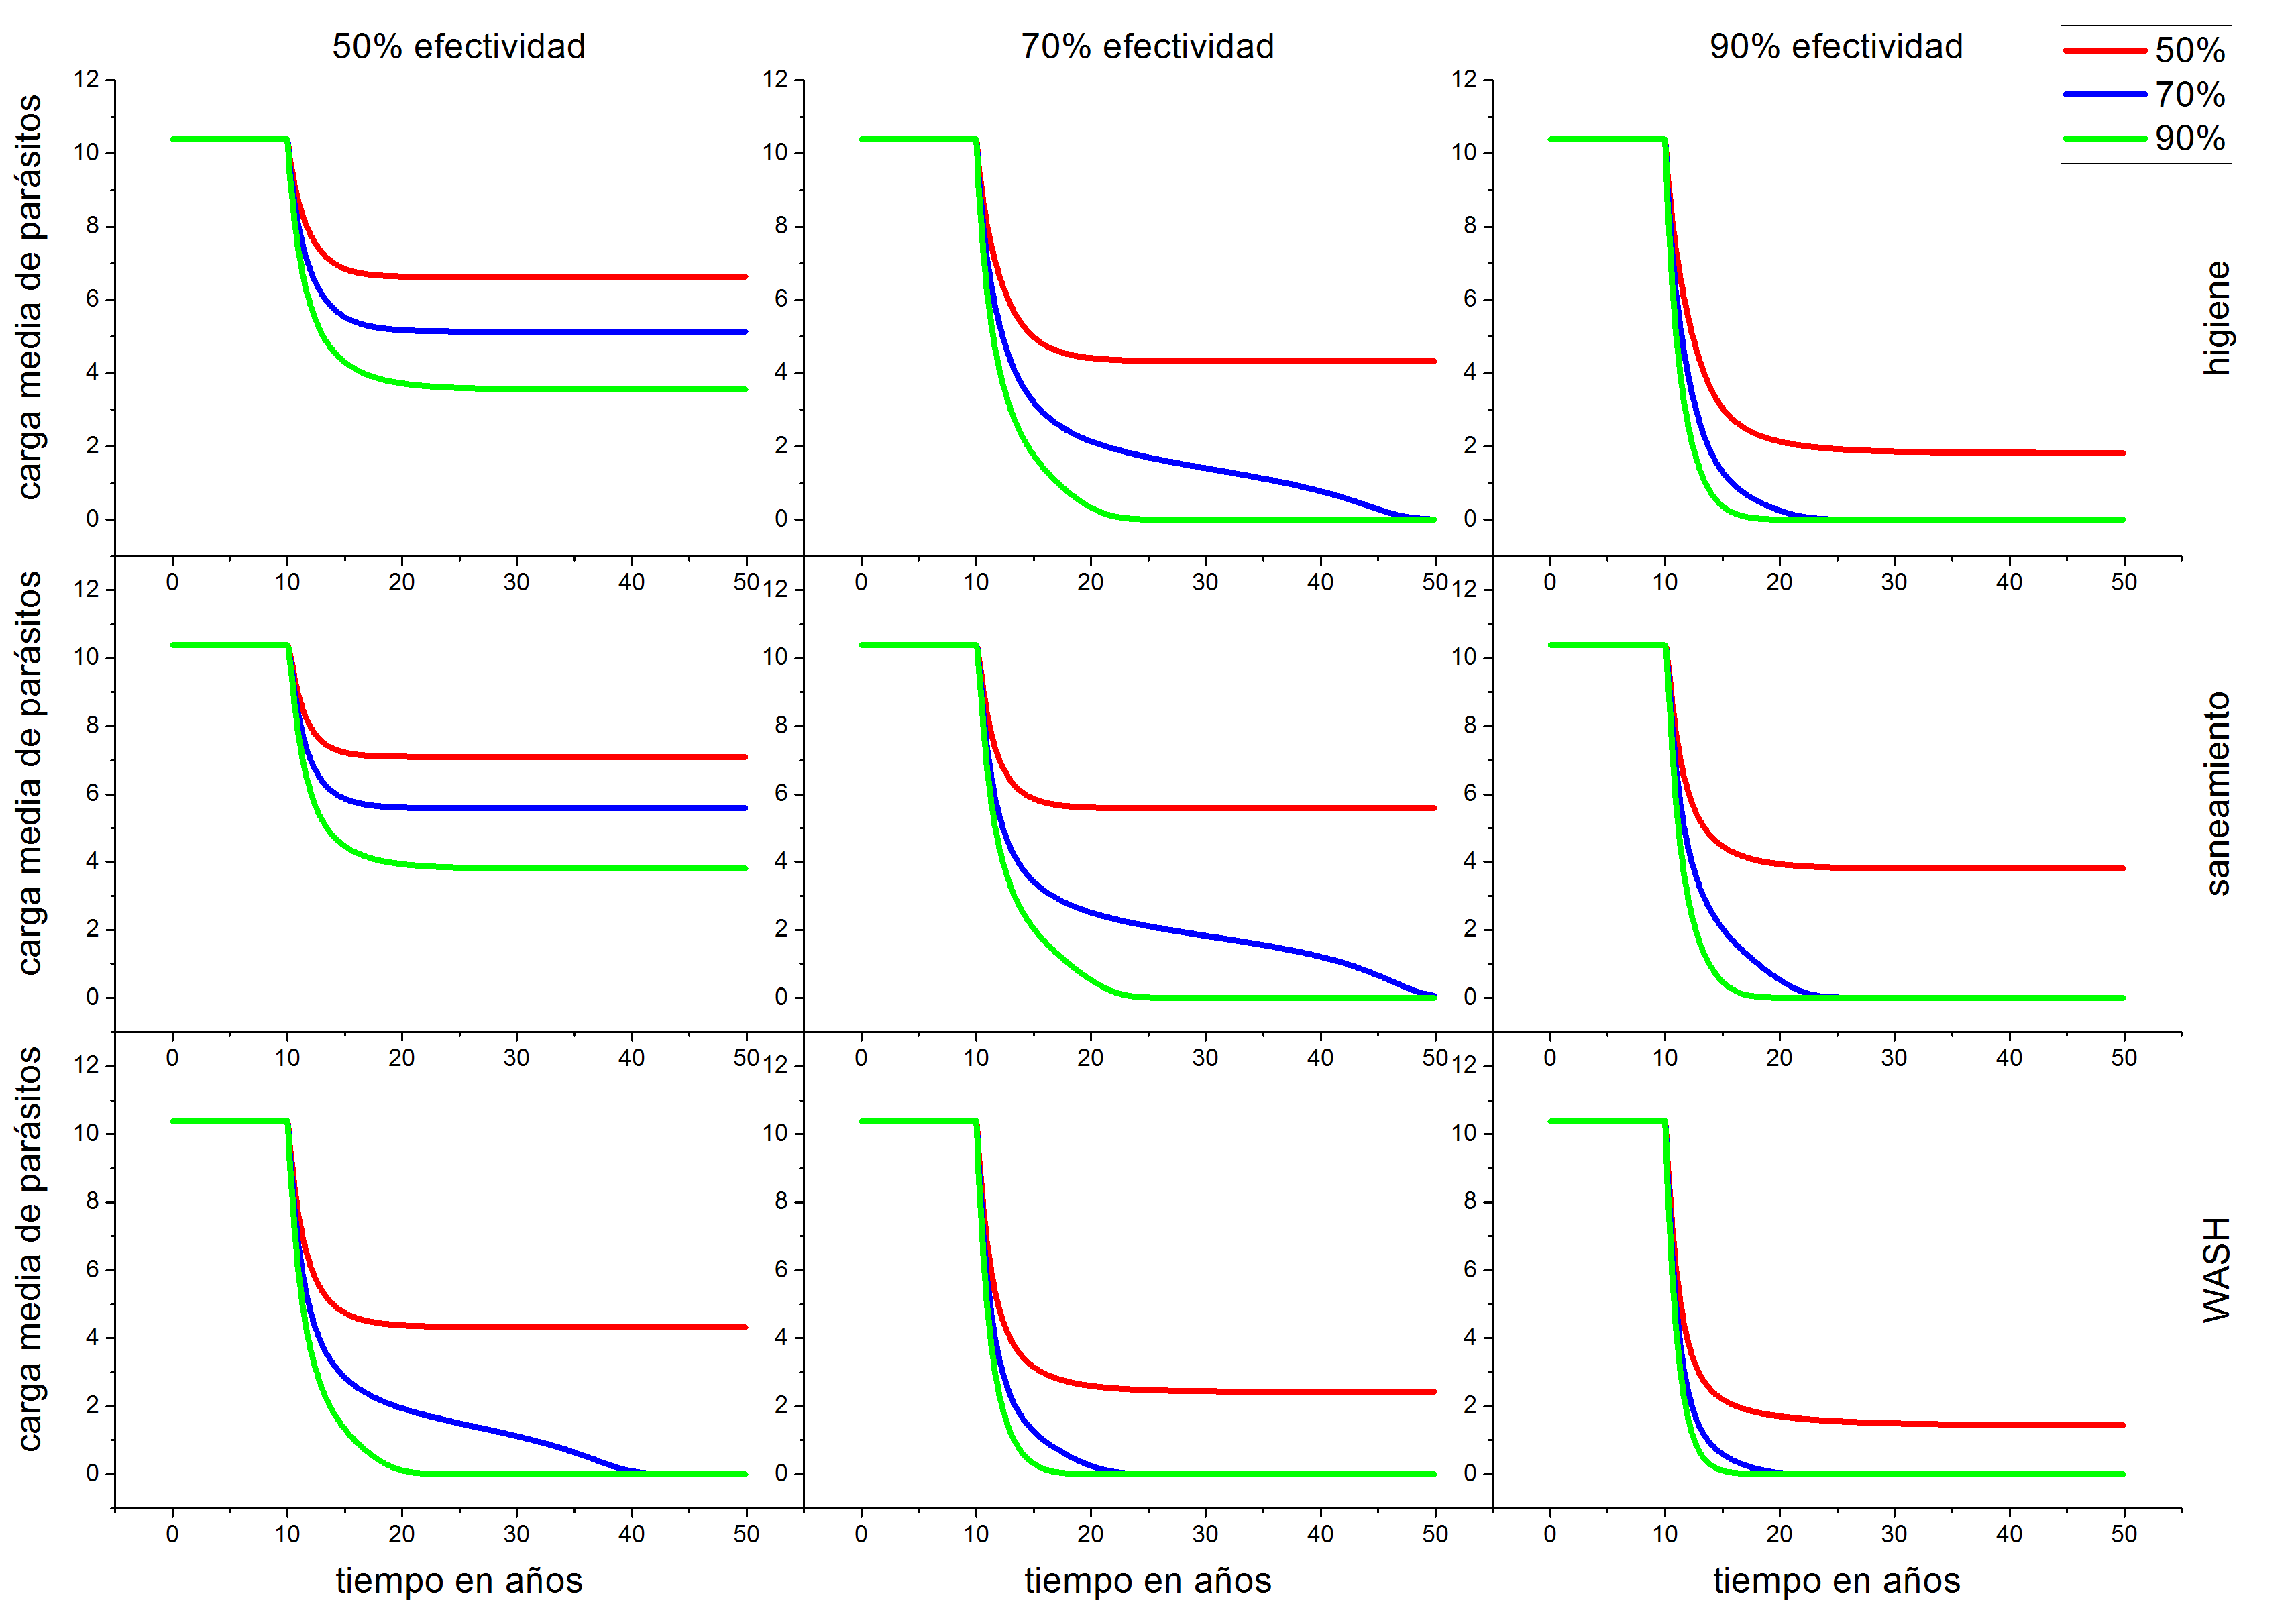
\includegraphics[width=.99\linewidth]{fig1}
		%\includegraphics[width=.99\linewidth]{model1conjuntov2}
		\caption{Series de tiempo de la cargas media de parásitos para las diferentes modalidades de intervenciones WASH (filas) contra diferentes niveles de efectividad (columnas) aplicadas a distintos porcentajes de la población (curvas de colores)}
		\label{fig:model1conjunto}
	\end{figure}

	De las simulaciones podemos observar (ver columna izquierda de la Figura \ref{fig:model1conjunto}) 
	%en la columna izquierda de la Figura \ref{fig:model1conjunto} 
	que suponiendo una efectividad del 50\% ($e_H=0.5$ y $e_S=0.5$), la cual suponemos la más realista, realizar intervenciones de higiene o saneamiento incluso al 90\% de la población (curva verde) no permite la erradicación de la infección. Sin embargo las intervenciones WASH (higiene + saneamiento) si permiten esta eliminación en unos 30 años cuando se aplica a un 70\% de la población (curva azul) y en unos 10 años cuando se aplica a un 90\% (curva verde). 
	
	Por otro lado si suponemos una efectividad del 70\% (ver columna central de la Figura \ref{fig:model1conjunto}). 
	%se requiere una eficiencia de recursos el escenario más conveniente consiste en suponer una efectividad del 70\% (columna central). 
	Donde suponemos que para conseguir este nivel de efectividad la población a tratar deber ser capacitada, concientizada y controlada (por ejemplo por agentes sanitarios) en el uso de higiene y saneamiento durante todo el periodo hasta la eliminación. 
	Si realizamos intervenciones de 
	%solo se puede proveer 
	higiene o saneamiento, el tiempo requerido para lograr cortar la transmisión depende de los porcentajes de la población tratada. Cuando un 70\% de la población (curva azul) tiene acceso a higiene o saneamiento, la erradicación de la infección se alcanza alrededor de los 40 años, mientras que cuando ese porcentaje sube a 90\% (curva verde) la erradicación se alcanza cerca de los diez años.
	
	%En este escenario si solo se puede proveer a la población únicamente de higiene o saneamiento la erradicación alrededor de los 40 años se consigue con la implementación de un 70\% de la población (curva azul) y en un poco más 10 años para un 90\% (curva verde). 
	
	Otro aspecto importante por mencionar es que en ningún escenario la erradicación se consigue tratando solamente al 50\% de la población (curva roja), incluso suponiendo una efectividad poco realista cercana a uno (90\%) permite esta erradicación (columna derecha).  
	
	
	
	\section{Discussion and Conclusions}
	%What is your most important finding?
	
	%{\color{red}
	
	En este trabajo, presentamos 
	modelos matemáticos deterministas y estocásticos para la dinámica de transmisión de las geohelmintiasis en poblaciones heterogéneas.  Estos modelos nos permiten evaluar el impactos de las intervenciones  WASH y PDM sobre la carga media de parásitos y poder determinar el periodo de eliminación de la infección
	 
	%modelos matemáticos deterministas y estocásticos para la dinámica de transmicion de las geohelmintiaisis. ESte estudio utiliza tanto modeos deterministas como esto casticos pata evaluar el impactos de las intervenciones  WASH y PDM sobre la carga media de parásitos y logras la eliminacion de la infecccion  
	
	Los modelos analizados muestran que la reducción de la carga media de parásitos y el periodo de eliminación de la infección dependen fuertemente de los parámetros:  proposición de la población con WASH ($p$) , efectividad de WASH ($e$) y el número de rondas de los tratamientos. Los parámetros $p$ y $e$ representan las características propias de las intervenciones WASH. 
	Mientras que el número de rondas de los tratamientos es una característica de los PDM. Los parámetros: proporción de la población con tratamiento ($g$), eficacia del tratamiento ($h$) propios de los PDM también impactan en la reducción de la carga media de parásitos y el periodo de eliminación del infección como se muestra en los trabajo \cite{anderson2014coverage,truscott2014modeling}, sin embargo aquí los valores de estos parámetros de encuentran fijos.     
	%proposición de la población con tratamiento ($g$), eficacia del tratamiento ($h$) y el número de rondas del tratamiento. 
	
  
	Para una población %, de niños (entre 2 y 14 años) y adultos (mayores de 15 años), 
	donde la tasa de contacto y aporte al reservorio de niños (entre 2 y 14 años) es el doble de los adultos (mayores de 15 años), este análisis determina que   
	%De este análisis encontramos que para el caso 
	%de una población %, de niños (entre 2 y 14 años) y adultos (mayores de 15 años), 
	%donde la tasa de contacto y aporte al reservorio de niños (entre 2 y 14 años) es el doble de los adultos (mayores de 15 años).   
	las intervenciones WASH permiten la erradicación de la infección para la modalidad  higiene + saneamiento a los 13 años de la implementación, para los valores $(p,e)=(0.7,0.7)$. Para las otra modalidades (higiene , saneamiento) no se consigue la eliminación. Para el caso de las intervenciones conjuntas WASH y PDM, con tratamientos anuales ($\tau=1$). La erradicación de la infección se consigue a los 13 y 8 años de la implementación, para los valores $(p,e)=(0.5,0.5)$ y $(p,e)=(0.5,0.7)$  respectivamente. 
	Para el modelo basado individuos con intervenciones conjuntas WASH y PDM, y tratamientos anuales ($\tau=1$). 
	La erradicación de la infección se consigue a los 20 años de la implementación con un probabilidad superior al 60\%, para los valores $(p,e)=(0.5,0.7)$. Mientras que para los 10 años de rondas de tratamientos la erradicación se consigue con una probabilidad menor al 10\%.
	
	La principal limitación de este trabajo es no contar con datos de campo que respalden los valores de los parámetros $p$ y $e$ asumidos en este trabajo. Esto se debe a la escasez de trabajos que puedan medir bien el impacto de las intervenciones WASH sobre poblaciones con geohelmintiasis. 
	
	
	En conclusión, mostramos que el impacto de las intervenciones WASH en la transmisión de las geohelmintiasis depende en gran medida de la modalidad de la intervención WASH, proporción de la población con intervención , efectividad de la intervención.  
		%Además, el impacto de WASH es difícil de medir en el contexto de los programas de desparasitación en curso.
		%Aún así, m
	Para el caso de los PDM, mostramos un claro beneficio adicional de las intervenciones WASH para mantener los avances logrados por los PDM a largo plazo, de modo que los PDM pueden reducirse o incluso detenerse por completo. 
	Todo lo anterior respalda como medida de control de las geohelmintiasis la
		%las políticas de 
	implementación conjunta de
		%la noción de que las políticas de 
	WASH y PDM.
	
		
		%En conclusión, mostramos que el impacto de las intervenciones de WASH en la transmisión de STH depende en gran medida de la especie de gusano, la modalidad de WASH y la aceptación y eficacia de la intervención. Además, el impacto de WASH es difícil de medir en el contexto de los programas de desparasitación en curso. Aún así, mostramos un claro beneficio adicional de WASH para mantener los avances logrados por PCT a largo plazo, de modo que PCT puede reducirse o incluso detenerse por completo. Todo lo anterior respalda la noción de que la política de WASH y PCT debe integrarse
	%} 
	
	
	\section*{Aknowledgements}
	
	This work was partially supported by grant CIUNSA 2018-2467. JPA is a member of the CONICET. GML is a doctoral fellow of CONICET.
	
	\section*{Conflict of Interest}
	
	The authors have declared no conflict of interest.
	
	
	%Reference
	\bibliographystyle{apa}
	\bibliography{biblio}	
	
	
	\appendix
	\section{Appendix}
	\subsection{Equilibria and Basic Reproduction Number}\label{subsec:apendice-model1}
	Considerando el análisis de estabilidad para el siguiente sistema 
	\begin{equation}
	\begin{split}
	\dfrac{dM_1}{dt}&=\beta_1 L - (\mu_H+\mu_M) M_1\\%\notag es para no tener numero en ecuacion
	\dfrac{d M_2}{dt}&=\beta_2 L - (\mu_{H}+\mu_M) M_2\\
	\dfrac{dL}{dt}&=\sigma \alpha \lambda \left[ \rho_1 \pi_1 M_1 F(M_1)+ \rho_2 \pi_2 M_2 F(M_2) \right]   - \mu_L L 
	\end{split}
	\end{equation} 
	Suponiendo una situación de equilibrio para el reservorio $L$, obtenemos que 
	\begin{equation}
	L^*=\frac{ \sigma \alpha \lambda}{\mu_L}  \sum_i  \rho_i \pi_i M_i F(M_i) 
	\end{equation} 
	y reemplazado esto en el resto de las ecuaciones del sistema inicial obtenemos las siguiente ecuación para la dinámica de la carga media $M$ de la población total de hospedadores 
	\begin{equation}
	\begin{split}
	\dfrac{dM}{dt}=  \frac{ \sigma \alpha \lambda}{\mu_L} \sum_i \beta_i \pi_i \sum_j  \rho_j \pi_j M_j F(M_j)  -(\mu_{H}+\mu_M) M%\notag es para no tener numero en ecuacion
	\end{split}
	\end{equation}
	Suponiendo el diferencial en cero, la carga media de parásitos en equilibrio, $M^*$, para la población total
	viene dada por
	\begin{equation}
	\sum_j \frac{ \sigma \alpha \lambda \rho_j}{\mu_L(\mu_{H}+\mu_W)} \left( \sum_i \beta_i  \pi_i \right) F(M^*_j) \pi_j M^*_j - \sum_i  \pi_i M^*_i=0 
	\end{equation}
	Esta no es una expresión explícita de los equilibrios $M_i^*$. Por lo tanto, el valor de los equilibrios solo se pueden resolver numéricamente. 
	Una condición de equilibrio para las cargas medias de cada grupo $j$ viene dada por 
	\begin{equation}\label{eqequilibrio}
	F(M^*_j)=1/R_{0j}
	\end{equation}
%	\begin{equation}
%	R_{0\rho}=\frac{\sigma \alpha \lambda }{ \mu_L (\mu_H+\mu_M)} (\beta \pi + \hat\beta \hat\pi)\rho
%	\end{equation}
%	donde $R_{0\hat\rho}$ y $R_{0\rho}$ es la contribución del grupo provisto y no provisto de agua y saneamiento respectivamente, para más detalles ver Apéndice (poner referencia).
%	
%	donde $\beta_1=\beta$, $\beta_2=\beta(1-\epsilon_A)$, $\rho_1=\rho$ y $\rho_2=\rho(1-\epsilon_S)$.
	donde definimos por $R_{0j}=\frac{ \sigma \alpha \lambda \rho_j}{\mu_L(\mu_{H}+\mu_M)} \sum_i \beta_i \pi_i $ al número reproductivo básico propio de cada grupo $j$ que es el número de hembras adultas que surgen 
	%en la población total del hospedador 
	de una hembra adulta de un hospedador del grupo $j$ en ausencia de los efectos de la denso-dependencia y la probabilidad de apareamiento. 
	Para esta situación de equilibrio obtenemos que la carga media de parásitos de cada grupo $j$ viene dada por $M_j^*=\frac{\beta_j}{\sum_i \beta_i \pi_i}M^*$.
	El número reproductivo básico general $R_0$ para la población total de parásitos esta dado por %\cite{diekmann2012mathematical}
	\begin{equation}\label{valorR0}
	R_{0}=\frac{\sigma \alpha \lambda}{\mu_L (\mu_{H} + \mu_W) }\sum_i \rho_i \beta_i  \pi_i 
	\end{equation}
	donde suponemos la ausencia de los efectos de la denso-dependencia y la probabilidad de apareamiento.
	
	Para los casos trabajados en la sección \ref{sec:model1} recordemos que
	\begin{equation*}
	\beta_1=\beta,\quad \beta_2=\beta(1-e_{H}),\quad \rho_1=\rho,\quad \rho_2=\rho(1-e_{S}),\quad \pi_1=1-\pi, \quad \pi_2=\pi 
	\end{equation*}
	donde para el caso 1 suponemos $e_{S}=0$ mientras que para el caso 2 suponemos $e_{H}=0$. 	 
	 
\end{document}
